\chapter{SAP}
\label{Kapitel:Einleitung}

SAP NetWeaver Business Intelligence (kurz: SAP BI) (vormals: Business Information Warehouse, kurz BW) ist die Data-Warehouse-Anwendung (kurz DW) der SAP AG und Teil von SAP NetWeaver. BW besteht unter anderem aus Komponenten zum Datenmanagement (Data Warehousing Workbench), zur Definition von Benutzerabfragen über einen OLAP-Prozessor (Business Explorer, kurz BEx), aus einer Data-Mining-Umgebung (Analyseprozessdesigner, kurz APD) und einer Komponente zur Kontrolle der Ladeprozesse. Die derzeitige Version des SAP Business Intelligence hat die Releasenummer 7.3 und ist Teil des SAP NetWeaver 7.3. 
Q: \url{http://de.wikipedia.org/wiki/SAP_NetWeaver_Business_Intelligence}


\section{Unterkapitel}
\label{Abschnitt:Motivation}




\begin{figure}[H]
    \centering
    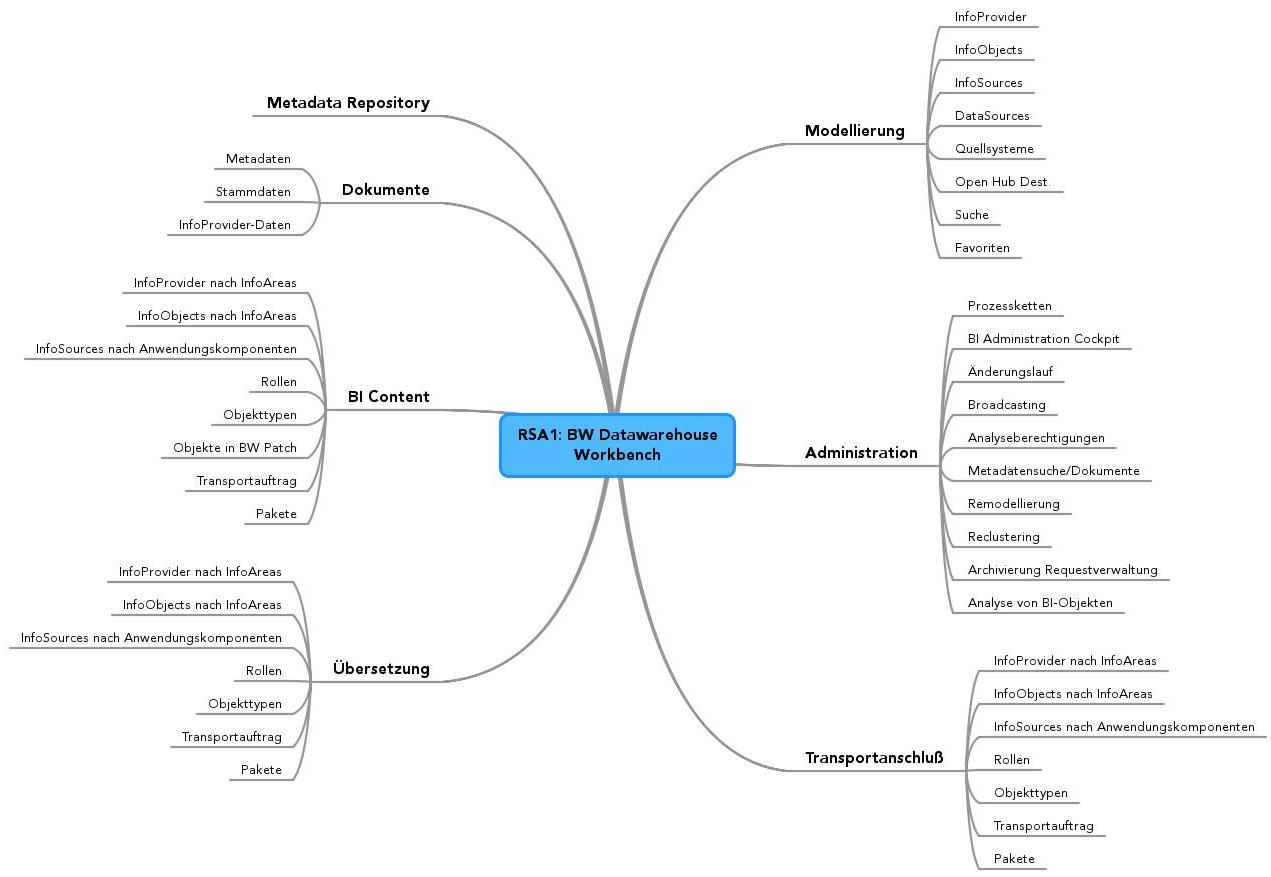
\includegraphics[width=1\textwidth]{files/RSA1Mindmap}
    \caption{Übersicht über RSA1}
    \label{pic:DWOverview}
\end{figure}





Text

\chapter{Modellierung}
> RSA1\\



We start our discussion by looking at the BW Administrator Workbench (transaction RSA1) – The administrator workbench is the central cockpit used for the administration of almost the entire BW system. As shown below, the RSA1 main screen can be divided into three general areas. The extreme left area, allows us to chose BW modelling components like Infoproviders, InfoObjects, InfoSources and DataSources. All of these components form part of the ETL (extraction, transformation and loading) concepts in SAP BW. Choosing any of the components, opens a view with a list of objects of the said type in the middle portion of the RSA1 screen. For example, if the component InfoProviders has been chosen, the main screen area shows a list of InfoProviders built in the specific BW installation. Individual BW components represented by different icons, the double diamonds being InfoAreas, the cubes being InfoCubes and the cylinders being Operational Data Store (ODS) objects. InfoAreas are not InfoProviders themselves but help to group similar InfoCubes under them. Other than InfoCubes, ODS objects, Multicubes and Infosets are other types of InfoProviders which can be encountered.
Right-clicking on an InfoProvider/InfoArea opens up a context menu which allows us to carry out different operations on the said object. For example we can create a new InfoProvider or change/display an existing one. The details of the chosen InfoProvider is now displayed in the right-most portion of the screen.

An InfoCube in general is made up of a number of information units called InfoObjects. These store data about the objects that are reported on. We can display a list of infoobjects defined in the system by choosing the InfoObjects option from the left hand screen as shown below. A right click on an individual InfoObject and following the options in the context menu allows us to display/change details for an InfoObject. InfoObjects can be of two types, Characteristics and Keyfigures. For example an InfoCube which stores sales data will store data about Customers. In this case, Customer is an characterististic which is part of the sales cube. Monthly unit of sales or similar data will be a keyfigure. As we can appreciate, Characteristic and Keyfigures store different kinds of data. They appear differently in reports and are secured through means. From the security standpoint, the fact whether we can selectively control access to an InfoObject is controlled by the contents of the Authorization Relevant flag in the explorer tab for an InfoObject. In the screen below, InfoObject 0COSTCENTER is marked as authorization relevant.

InfoObjects in turn can also have their own attributes. Following the earlier example, the InfoObject Customer would have attributes like Customer Address, Bank Details, Tax number etc. The following screen shows the the attributes of InfoObject 0COSTCENTER. We can observe that the attributes can be two types, Display attributes (DIS) and Navigational Attributes (NAV).Security for a navigational attribute can be enabled by switching on the authorization relevant flag shown in the screen below. The latest version of BW (BI 7) allows Navigational Attributes to be secured differently from the base InfoObject. %Thus BI 7 can allow different security for InfoObject 0COMP_CODE and the navigational attribute 0COSTCENTER_0COMP_CODE depending on requirements. 

Metadaten erstellen\\
InfoProvider, InfoObject, InfoSource\\
PSA :Persistent Staging Area
Die Persistent Staging Area (dt. dauerhafter Bereitstellungsbereich, kurz PSA) ist in SAP BW eine Datenbanktabelle, die der Struktur (Transferstruktur) der Schnittstelle zum Quellsystem (meistens ein SAP R/3-System) entspricht. In dieser Tabelle werden die Daten beim Datenladen abgelegt, wenn dies in den Einstellungen zum Ladelauf (Reiter Verarbeitung des InfoPackages) so angegeben ist.

Die PSA-Tabelle wird je Datenquelle (DataSource) und Quellsystem angelegt, da die Datenquellen unterschiedlich aufgebaut sein können. Die Quelldaten werden unverändert im PSA abgelegt und erst dann anhand von Transferregeln verarbeitet und danach in einer weiteren Struktur (Transformation) zum Laden in die Datenziele bereitgestellt. Somit bestehen die Originaldaten im BW weiterhin und können zum Neuaufbau zum Beispiel von Merkmalen (InfoObjects), Datenwürfeln (Infoprovidern) und DSO-Objekten verwendet werden. Es ist kein neuerlicher Ladelauf aus dem Quellsystem erforderlich. Die PSA-Tabelle kann also als Zwischenspeicher verwendet werden, jedoch nicht als Datenquelle, auf die direkt Auswertungen zugreifen können. Des Weiteren kann beim Auftreten von fehlerhaften Daten aus dem Quellsystem im PSA eine manuelle Datenbereinigung durchgeführt werden.

Die PSA-Tabelle kann in regelmäßigen Abständen gelöscht werden, indem Löschprozess in einer Prozesskette eingeplant wird. Dies erfolgt je Datenquelle (DataSource) und Quellsystem. \\ 
Aus PSA Teil direkt aus Wikipedia

\chapter{Monitoring}
>RSMON\\
Hier können Daten und Datenladeprozesse überwacht werden.

\chapter{Buisness Content}
> RSORBCT\\
Eine Art Informationsdatenbank?
- Ist vorkonfiguriert und basiert auf standardmodellen und metadaten

\chapter{Metadata Repository}
>RSOR\\
Zeigt alle Metadaten in Html an und verknüpft sie miteinander. Volle HTML funktionalität (Export und Graphiken usw.)\\

Gute Quelle:
\url{https://help.sap.com/saphelp_nw70/helpdata/en/80/1a60cae07211d2acb80000e829fbfe/content.htm?frameset=/en/a8/6b023b6069d22ee10000000a11402f/frameset.htm&current_toc=/en/e3/e60138fede083de10000009b38f8cf/plain.htm&node_id=53&show_children=true#jump56}




